\graphicspath{{solutiondevelopment/fig/}}

\chapter{Solution development}
\label{chap:solutiondevelopment}
The goal of this project is to develop a tool for calculating the low frequency mean square flux noise figure given a SQUIDs geometry with the use of the software package InductEx. In \cite{fluxNoiseSquidsStevenAnton} the authors propose a framework for implementing such a tool but then only applied the method to a square washer. As pointed out in \cite{fluxNoiseSquidsStevenAnton} the other numerical technique suffers from performance and resolution problems. This section will serve to communicate the design effort by systematically breaking down the problem and motivating design decisions along the way. I will start by first identifying the design requirements.

\section{Design goals}
In section \ref{chap:litreview} it was made clear that the origin of the low frequency noise is still unknown. The S.M. Anton et al. pointed concluded \cite{fluxNoiseSquidsStevenAnton} by remarking on the flexibility of his numerical framework. It can readily be adapted, with only minor modifications to the framework, to account for a variety of different models. As such a major design requirement is to reflect the flexibility of the framework within the design of the tool.
The second and perhaps most obvious design goal is that the tool must be fast. The end user of such a tool is a SQUID designer. As discussed in chapter \ref{chap:litreview} the design of SQUID systems relies heavily on computational methods. The non-linear nature of the Josephson junctions makes analytical solutions to design problems not feasible. In such cases the designer often has to rely on an iterative approach to design.
The tool must be generalized to work on any geometry one might give it.
The last design goal is to use TetraHenry for the calculation of the magnetic flux density. 

\section{High Level System Design}
The project calls for the development of 2 independent modules. The first module must implement mesh refinement around regions of rapidly varying currents across mesh nodes. The second module must implement the numerical framework as described by \cite{fluxNoiseSquidsStevenAnton} using the simulation results from InductEx and TetraHenry. \par
To understand the role the tool will play one must first understand the basic interactions a user might have with the software package. One must also understand what each entity requires as input and what its outputs are. Figure \ref{fig:Inductexproc} summaries this and figure \ref{fig:ProcessFlow} shows how each module interacts with this process.
\begin{figure}[h]
    \centering
    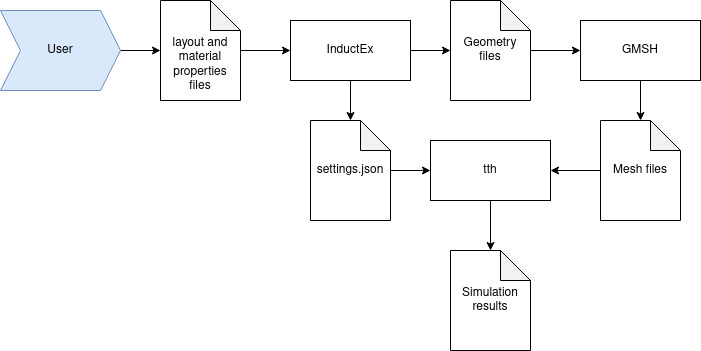
\includegraphics[width=0.8\linewidth]{Inductexproc}
    \caption{A process showing how the average user might interact with InductEx and TetraHenry. The figure also shows typical input and output files at each entity in the process.}
    \label{fig:Inductexproc}
\end{figure}
\begin{figure}[h]
    \centering
    \includegraphics[width=0.8\linewidth]{ProcessFlow}
    \caption{A process chart showing how the user interacts with InductEx as well as how each module will interact with this process.}
    \label{fig:ProcessFlow}
\end{figure}

\subsection{InductEx}
InductEx has gone through major changes since the publication of \cite{fluxNoiseSquidsStevenAnton}. InductEx is a powerful tool that supports a large feature set. Most of these features are not relevant to this project. I only require magnetic field calculations and current distribution for the surface of the conductor, so these features will mostly be ignored.

\subsection{GMSH}
GMSH is an open-source tool that is used to discretize geometry \cite{GMSH}. GMSH supports a scripting language to specify geometry before discretization. InductEx generates a file in this scripting language to be run through GMSH to generate a finite element mesh for use in TetraHenry. GMSH typically accepts a ".geo" file and outputs a ".msh" file. In GMSH you specify the geometry in a hierarchical fashion. You start by defining the lowest dimension elements and build up the geometry from there. In GMSH the lowest dimension entity is the point and is referred to as a "0 dimensional" entity. Higher dimensional entities are bounded by lower dimensional entities for example: A volume is bounded by a set of 2 dimensional surfaces. A surface is defined by a closed loop of 1 dimensional curves. A curve is defined by the 0 dimensional points. This fact will become useful in the design of the GMSH extraction module. GMSH entities are added to physical groups specified by the user. Physical groups are essentially just names for collections of mesh entities. The most common use of physical groups is to use them to define material properties. The implementation and use of physical groups depend on the context GMSH is used in. In TetraHenry physical groups are used to specify a number of things but most relevant to this project, it is used to specify the mesh entities to be used for field calculations. \par

\subsection{TetraHenry (TTH)}
TetraHenry is the numerical field solver that will be used to calculate the surface magnetic flux density. This project will interact directly with TetraHenry. Refer to appendix \ref{appen:settings} for the template ".json" settings file used. Depending on the setup of the simulation, TetraHenry will write the results to a folder titled output. When specified, TetraHenry will write the magnetic flux density to a "vtk" file as an unstructured grid. TetraHenry also supports a feature where a loop can be excited by specifying a "hole" port. This eliminates the problems \cite{fluxNoiseSquidsStevenAnton} had where the current distribution was distorted around the port where the test current is injected. 

\section{Detailed Design}
\subsection{Choice of programming language}
The visualisation tool kit (VTK) is an open-source modelling and visualisation tool kit. As TetraHenry reports simulation results in the VTK file format it is necessary that the language of choice supports the VTK library. Of the rich variety of programming and scripting languages available, few match the design requirements. The VTK library is only supported by python and C++. Python is a high level interpreted language and is often used for scientific computing. Python is very flexible but suffers from performance issues due to it being interpreted. C++ is a lower level compiled programming language that is generally regarded as a "fast" programming language. This is largely due to the fact that it does not have the overhead that comes with an interpreted language. In order to meet performance goals C++ will be used.


\subsection{The mesh optimisation module}
The idea behind mesh optimisation in this context is to reduce the number of mesh elements in the resulting mesh without compromising on the accuracy of the field calculations. In the work done by Anton et al. \cite{fluxNoiseSquidsStevenAnton} an older version of InductEx was used. This version of InductEx used filaments as mesh elements. In many optimisation problems the challenge is to find a solution to said problem under some constraint. The challenge in mesh optimisation is finding this constraint. The methods employed by the authors in \cite{fluxNoiseSquidsStevenAnton} involved finding the spline interpolation of currents between adjacent nodes. The constraint was then set such that the change in current between nodes cannot exceed a user specified threshold. If adjacent mesh elements are found where this is the case the mesh elements are divided using the spline interpolation to adhere to this constraint. The new mesh is then used to solve for the current distribution and the same process is repeated until it reaches the iteration limit or the solution converges on a stable mesh (no subdivisions are made). \par
The version of InductEx this project is designed to work with supports tetrahedral meshing which is a far superior approach. As previously mentioned, all meshing is done with GMSH and as such mesh optimisation of this nature will require some form of integration with GMSH. \par
In GMSH the longest side of a mesh element (triangle) is referred to as the characteristic length. The characteristic length essentially defines how finely a geometric model is meshed. The characteristic length is therefore closely related to the number of mesh elements in the resulting mesh. Clearly this is how the mesh must be optimized. The characteristic length of each mesh element must be chosen such that a finer mesh is generated where the current varies rapidly across mesh elements. GMSH does not allow for the direct specification of mesh element characteristic lengths. The characteristic length of each element is instead specified through the following methods: 

\begin{enumerate}
    \item By specifying the characteristic lengths at each point in the geometric model. If the "\textit{Mesh.MeshSizeExtendFromBoundary}" option is set to true, the characteristic length will be interpolated between the defining points, curves and surfaces.
    \item By specifying the number of mesh elements per rotation.
    \item By specifying mesh size fields.
    \item By specifying structured meshing constraints.
\end{enumerate}
Option 3 was chosen because it provides the most control over mesh sizes and is the closest to being able to specify individual mesh element sizes. \par
A field in GMSH refers to a post-processing view. A post-processing view can be used as a mesh size field by setting it as a background mesh. The problem reduces to finding an appropriate background mesh. There are 2 quantities that can be used to generate the background mesh. The two options are using the magnetic flux density or using the current density. The choice of current density was made as it is what ultimately determines the magnetic flux density thereby eliminated compounding error caused by calculating the magnetic flux density from a crudely approximated current density distribution.
\subsubsection*{The minimum relative change approach}
This implementation took the approach of \cite{fluxNoiseSquidsStevenAnton}. Instead of using a spline interpolation I opted for a linear interpolation for performance reasons. The implementation should be flexible in case different interpolation method is found to produce far superior results. \par
In this approach the VTK library is used to parse the current distribution file generated by TetraHenry. The task is to find a suitable characteristic length for each node in a mesh element to be written to the background field. The process is explained with reference to figure \ref{fig:meshopt}.
\begin{figure}[H]
    \centering
    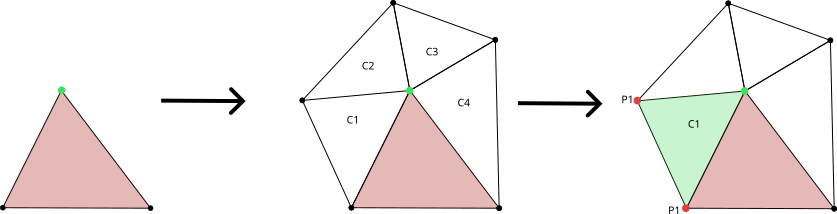
\includegraphics[width=0.9\linewidth]{meshopt}
    \caption{The figure shows the steps in the mesh optimisation algorithm when the current density is used to constrain mesh element sizes. Red region is the cell in the current iteration. The green point is the point being considered in the current iteration of looping through the points in the red region. The next step shows the mesh cells connected to the green point. The last step shows the points which will be compared to the green point. The process repeats from the second step until all cells have been explored and a maximum change of current density for the green point is found. The then algorithm reverts to the next point in the red cell and the process repeats.}
    \label{fig:meshopt}
\end{figure}
The algorithm starts by looping through every mesh element in the mesh. For a given point ($p$) in the mesh element, the VTK library can be used to find all the cells connected to point $p$. Each point in each cell is looped over to determine the maximum change in current density between point $p$ and a point connected to it. The change in magnitude between point $p$ and the point that gives the greatest change in $J$ is divided by the magnitude of the current density at point $p$ to give a percentage change in current density magnitude. The user specifies the minimum relative change allowable between adjacent nodes in the mesh. If the relative change exceeds this value it is subdivided by setting the characteristic length to a value such that, under a linear interpolation scheme and assuming that the line joining the points will be subdivided into segments equal to the characteristic length, the relative change never exceeds the minimum value between the 2 points. The values are then appended to the geometry file being optimised.

\subsubsection*{The non-linear mapping function approach}

To convert the magnitude of the current density to a characteristic length at each node a non-linear mapping is used. A linear approximation of a sigmoid function was chosen. The motivation for choosing a sigmoid function is it allows for the user to specify minimum and maximum mesh size while still interpolating between both boundaries. The approximation is used for performance reasons. Figure \ref{fig:sigmoid} shows the sigmoid and its linear approximation.
\begin{figure}[h]
    \centering
    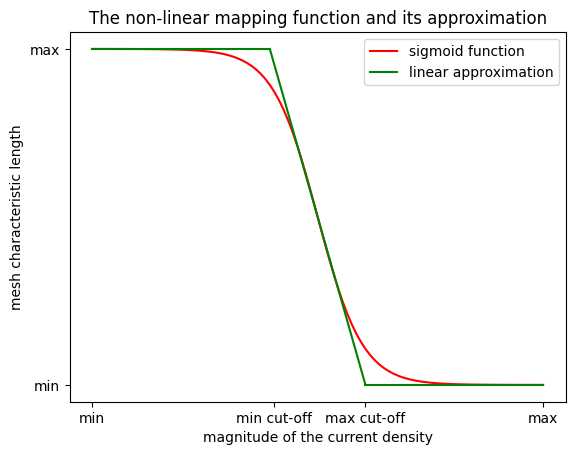
\includegraphics[width=0.5\linewidth]{sigmoid}
    \caption{A graph showing the sigmoid function with its linear approximation}
    \label{fig:sigmoid}
\end{figure}
The values that define the properties of the mapping are specified by the user. The user must specify the min cut-off, max cut-off, maximum magnetic flux density, minimum magnetic flux density, maximum characteristic length and minimum characteristic length. The module then loops through each point in the mesh and calculates the desired characteristic length from the mapping function. The background mesh is specified as a collection of triangles. Each triangle consists of three points where the characteristic length is set for each point. The background mesh is appended to the geometry file and GMSH is run to mesh the structure. 

\subsubsection*{The chosen approach}
The first option was chosen because the large number of parameters the user must specify to use the magnetic flux density is not convenient for automated testing. This is because after each mesh optimisation the values necessary to prevent over or under refinement of the mesh changes. The advantage of the non-linear mapping function approach is that it runs faster, and it provides more control over the optimized mesh. This opens the door to possible future investigations into combining the 2 approaches. 

\subsection{The noise extraction module}
This module is based on the work done by \cite{fluxNoiseSquidsStevenAnton}. This module will be implemented as a command line tool. The module receives the path to a VTK file which defines an unstructured grid and the total current circulating in the SQUID washer as command line arguments. The unstructured grid specifies the individual mesh elements that the surface of the SQUID washer in question consists of. Additionally, each node of each mesh element has a vector associated with it representing the magnetic flux density at the location of said node. \par
This module effectively implements equation \ref{eq:MSFNfromBfield} numerically. Expanding equation \ref{eq:MSFNfromBfield}:


\begin{equation}
    \langle \Phi ^2 \rangle = \frac{N\mu_B^2}{3I^2} \frac{\iint \Vec{B(\Vec{r})}\cdot\Vec{B(\Vec{r})} ds}{\iint ds}
    \label{eq:MSFNexpanded}
\end{equation}

Noting that in equation \ref{eq:MSFNexpanded} $N/\iint ds = \sigma$ and therefore the bottom integral can be eliminated \cite{fluxNoiseSquidsStevenAnton}. Next we discretize the integral: 
\begin{equation}
    \langle \Phi ^2 \rangle = \frac{\sigma\mu_B^2}{3I^2}\sum_{n}^{N_{\text{nodes}}}[\Vec{B}(\Vec{r_n})\cdot\Vec{B}(\Vec{r_n})]A_n
    \label{eq:MSFNdiscrete}
\end{equation}
In equation \ref{eq:MSFNdiscrete} $A_n$ refers to the area associated with the $n_{th}$ node. The method for determining $A_n$ is discussed at a later stage in the design. Similarly, $\Vec{r_n}$ refers to the vector position of the $n_{th}$ node in the unstructured grid. The basic algorithm then follows as such:
\begin{algorithm}
\begin{algorithmic}
    \State $N \gets \text{Number of points in grid}$
    \State $pts \gets \text{list of all points}$
    \State $A \gets $ list of all areas
    \State $i \gets 0$ 
    \While{$i < N$}
        \State $A_n \gets A[i]$
        \State $r_n \gets pts[i]$ 
        \State $\Phi^2 \gets \Phi^2 + \Vec{B}(\Vec{r_n})\cdot \Vec{B}(\Vec{r_n}) A_n$ 
    \EndWhile
    \State $\Phi^2 \gets \Phi^2 \cdot \frac{\sigma\mu_B^2}{3I^2}$ 
\end{algorithmic}
\caption{The algorithm for evaluating the discretized integral}
\end{algorithm}

% \subsection{Calculating the node areas}

\subsubsection*{The Choice of $\Vec{A_n}$}
Equation \ref{eq:MSFNdiscrete} shows that the calculation requires the weighted summation of the flux density over the surface. The resulting unstructured grid generated by TetraHenry associates each flux density vector with a node in the surface mesh. Figure \ref{fig:washerCloseUp} shows and example of what this looks like in practice. The challenge then is finding a scheme for choosing $A_n$.

\begin{figure}[h]
    \centering
    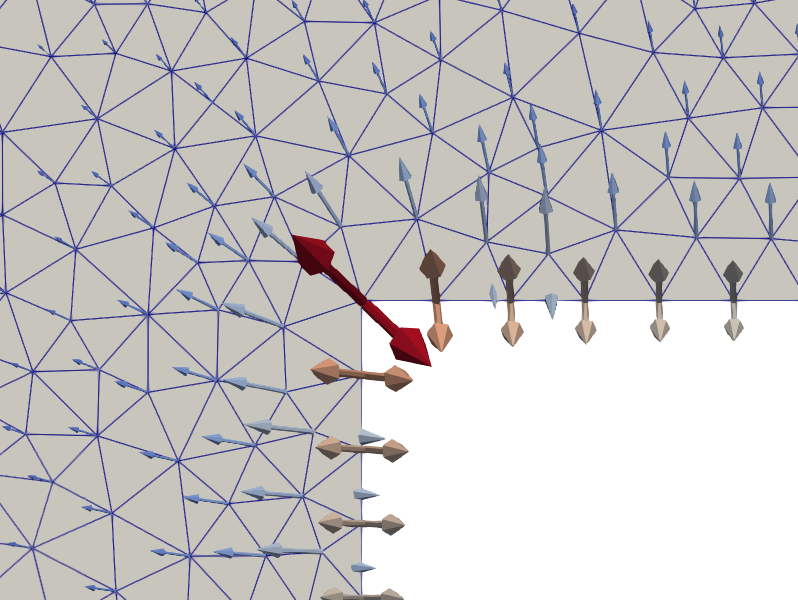
\includegraphics[width=0.5\linewidth]{washerCloseUp}
    \caption{A close up of a square washer showing the field calculations at each node in the triangular mesh.}
    \label{fig:washerCloseUp}
\end{figure}
To get some idea of what $A_n$ should look like we can investigate some of its properties. The first property of $A_n$ is expressed in equation \ref{eq:surfaceArea}.

\begin{equation}
    \text{Surface Area} = \sum_{n=0}^{N}A_n
    \label{eq:surfaceArea}
\end{equation}

The second property we would like from $A_n$ is that it minimizes the error caused by discretization. 

\begin{equation}
    ||\Vec{B_n} A_n - \iint\limits_{r \in A_n}\Vec{B}(\Vec{r})ds || = E
    \label{eq:surfaceError}
\end{equation}

It is evident from equation \ref{eq:surfaceError} that the error is $0$ when $\Vec{B}(\Vec{r}) = \Vec{B_n}$. This is not usually the case. If we assume that the mesh is fine enough such that $\Vec{B}(\Vec{r})$ varies slowly across adjacent mesh elements, we can say that the error is roughly proportional to the distance of a point in the region defined by $A_n$ to the mesh node to which $A_n$ belongs to. With this in mind we construct a new optimisation problem. \par 
Let $\Vec{X}$ be a metric space representing the surface area of the structure. We define a set of points $\Vec{P} \in \Vec{X}$ such that $\Vec{P_k}$ refers to the coordinates of the $k_{th} \in K$ node in the mesh. We would like to divide the metric space $\Vec{X}$ into $K$ regions such that each region is assigned the points closest to it thereby minimizing the error due to discretization. The $k_{th}$ region is denoted as $A_k$. Based on these arguments we can write down an objective function for this problem. The objective function quantifies the total error due to our choice of region at point $\Vec{x}$ defined by the function $t_k(\Vec{x})$.

\begin{equation}
    J = \iint \limits_{\Vec{x}\in\Vec{X}}\sum_{k}^{K}t_k(\Vec{x})||\Vec{x}- \Vec{P_k}||^2ds
    \label{eq:objFunc}
\end{equation}
The problem reduces to finding the choice of $t_k(\Vec{x})$ that minimizes $J$. The function, $t_k(\Vec{x})$ can be understood as a "label" function. It is 1 for every point $\Vec{x}$ we choose to be in region $k$ or 0 if the point is not in region $k$. The obvious choice for minimizing the sum is to set $t_k(\Vec{x})$ to zero for all $K$ regions except for the region where the distance to the point $\Vec{P_k}$ is at a minimum. Mathematically this can be expressed by equation \ref{eq:tk}

\begin{equation}
    t_k(\Vec{x}) = 
    \begin{cases}
        1 & \quad \text{If} \quad k = argmin_j\{||\Vec{x} - \Vec{P_j}||^2\}  \\
        0 & \quad \text{Everywhere else} \\
    \end{cases}
    \label{eq:tk}
\end{equation}
Recalling the definition of the Voronoi region defined in the metric space $\Vec{X}$ with the distance function $d$ and sites defined by the points $(\Vec{P_k})_{k \in K} $: 
\begin{equation}
    \Vec{A_k} = \{\Vec{x} \in \Vec{X}|d(\Vec{x},\Vec{P_k}) \leq d(\Vec{x},\Vec{P_j})\forall  j \neq k \}
    \label{eq:voronoi}
\end{equation}
If we choose the distance function in equation \ref{eq:voronoi} to be the euclidean distance we see that the regions that minimize the objective function is the Voronoi regions. \par
Choosing $A_n$ to be the Voronoi regions is a good choice not only because under the assumptions made, it minimizes the objective function but also because the triangular mesh is a Delaunay triangulation. The Delaunay triangulation is the geometric dual of the Voronoi tessellation meaning if you have the Delaunay triangulation, you have the Voronoi tessellation. This choice for $A_n$ is therefore computationally efficient. This choice also adheres to the first property we expected of $A_n$ as the Voronoi regions partition the metric space $\Vec{X}$. \par
The mesh generated by GMSH can be used to directly compute the points that define the Voronoi regions. An example is shown in figure \ref{fig:voronoi}. 

\begin{figure}[h]
    \centering
    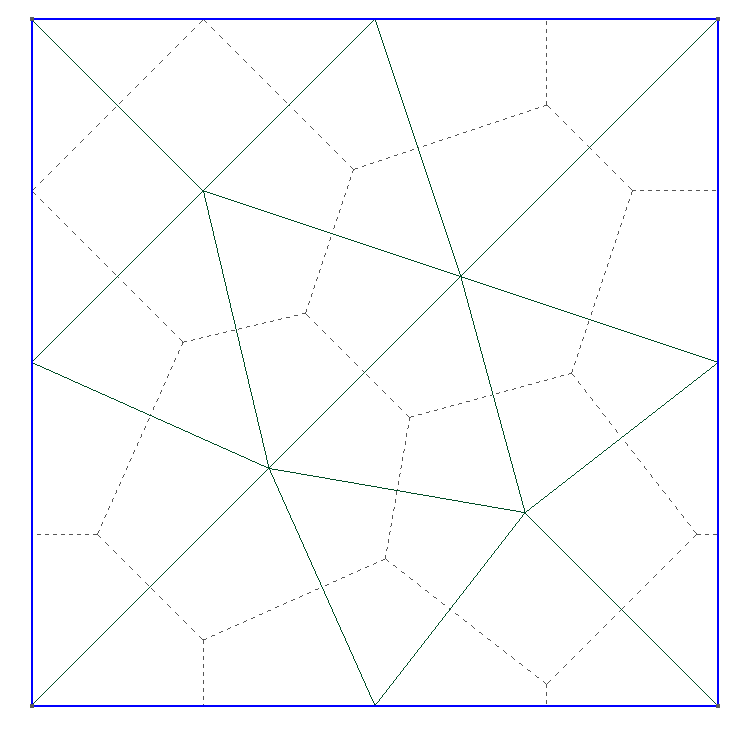
\includegraphics[width=0.3\linewidth]{voro}
    \caption{The Delaunay triangulation is shown. The triangular mesh is the solid lines. The Voronoi cells are constructed out of the dashed lines. This figure was generated with GMSH \cite{GMSH}}
    \label{fig:voronoi}
\end{figure}

These points that define the vertices of the Voronoi cells are the circumcenters of the Delauny triangulation. The algorithm follows:

\begin{algorithm}[H]
    \begin{algorithmic}
        \State $ CellList \gets $[ ]
        \For{Node $n$ in Nodes} 
            \State $C \gets $ getPointCells($n$)
            \State $V_{\text{points}} \gets $[ ] 
            \For{Cell $c$ in $C$}
                \State $P \gets $ getCellPoints($c$)
                \State $cc \gets $ computeCircumCenter($P$)
                \State $V_{\text{points}}$.pushPoint($cc$)
            \EndFor
            \State $CellList$.pushNewCell($V_{\text{points}}$)
        \EndFor
    \end{algorithmic}
    \caption{The algorithm for evaluating the discretized integral}
\end{algorithm}
When the loop exits the $CellList$ contains all the points that define the Voronoi cells. The VTK library is used to parse the simulation results. It supports optimized methods for retrieving all cells connected to a node as well as methods for fetching the points belonging to a cell. Given the position vectors $P_1$, $P_2$ and $P_3$ of the vertices of the triangle, the circumcenter ($P_c$) of a triangle arbitrarily oriented in space can be calculated using equation \ref{eq:BaryCenter}.

\begin{equation}
    P_c = \alpha P_1 + \beta P_2 + \gamma P_3
    \label{eq:BaryCenter}
\end{equation}
where 
\begin{table}[h]
    \centering
    \begin{tabular}{l}
        $\alpha = \frac{|P_2 - P_3|^2(P_1-P_2)\cdot(P_1-P_3)}{2|(P_1-P_2)\times (P_2 - P_3)|^2}$\\
        \\
        $\beta  = \frac{|P_1 - P_3|^2(P_2-P_1)\cdot(P_2-P_3)}{2|(P_1-P_2)\times (P_2 - P_3)|^2}$\\
        \\
        $\gamma = \frac{|P_1 - P_2|^2(P_3-P_1)\cdot(P_3-P_2)}{2|(P_1-P_2)\times (P_2 - P_3)|^2}$\\
    \end{tabular}
\end{table}
The perpendicular bisectors of the sides of a triangle intersect at the circumcenter, so the midpoint of each side is added to the point list of a Voronoi cell. This does not influence the shape of the cell as adjacent triangles share a side and, by the definition of a perpendicular bisector, share a perpendicular bisector. The added point is therefore collinear with the line joining adjacent circumcenters. This is done to satisfy boundary conditions. The effect of this will be discussed in more detail when the ordering of points in 3 dimensions is discussed.
\subsubsection*{The shoelace algorithm}
Now that an algorithm for choosing $A_n$ has been selected the next step is to calculate the area. If we consider an ordered set of coplanar points that define a convex N-sided polygon, the surface area of this polygon can easily be calculated using the shoelace algorithm. One property of this specific Voronoi tessellation is that the regions are always defined by convex polygons making this assumption very reasonable. Equation \ref{eq:Shoe} calculates the area given an ordered list of coplanar points $v_0, v_1, \dots, v_{N}$.

\begin{equation}
    A = \frac{1}{2}|\sum_{i=1}^{N}(v_i - v_0) \times (v_{(i+1) \% N} - v_0) |
    \label{eq:Shoe}
\end{equation}
The assumptions that all points in the Voronoi cell are coplanar and that all points are ordered does not hold. On curved surfaces or on surface edges there is more than 1 plane that the points in the cell belong to. Focusing on the assumption that all points in the Voronoi cell are co-planar, the algorithm must be able to group the points into sub cells that are coplanar. The assumption that the points are ordered will be addressed in the next section. \par
The points are read in using the VTK library triangle by triangle. Each triangular cell is read in through the "getPointCells" method. This method returns the cells that all share a point specified by an argument passed to the method. The shared point is used as the reference point. The reference point is then subtracted from every other point in the cell. The cross product of the resulting vectors is the normal to the plane that the cell is in. Due to the non-commutative nature of the cross product the order of the vectors matter. To account for this the implementation will consider both $a_n$ and $-a_n$ as the same plane. Where $a_n$ refers to a unit vector normal to the plane. The last modification that must be made is the addition of the reference point to the geometry of each sub cell. The implementation will add the reference point to each sub cell if the number of unique planes that the reference point belongs to is greater than 1. Figure \ref{fig:voroComp} demonstrates the need for this.

\begin{figure}[h]
    \centering
    \begin{subfigure}[b]{0.45\textwidth}
        \centering
        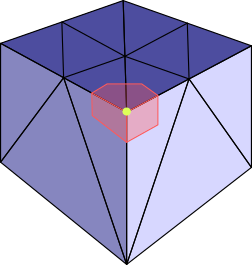
\includegraphics[width=0.5\textwidth]{vorocube}
        \caption{The Voronoi tessellation with the inclusion of the reference point}
    \end{subfigure}
    \hfill
    \begin{subfigure}[b]{0.45\textwidth}
        \centering
        \includegraphics[width=0.5\textwidth]{vorocubeWrong}
        \caption{The Voronoi tessellation without the inclusion of the reference point}
    \end{subfigure}
    \caption{The figure shows two examples of a cube. The surfaces have been meshed into triangles. The red lines indicate the boundaries of the Voronoi cell and the shaded region shows the Voronoi cell region. The yellow dot indicates the current reference point.}
    \label{fig:voroComp}
\end{figure}
The shoelace algorithm can then be performed on each individual sub cell to calculate the total area associated with a node. Figure \ref{fig:voroComp} also shows why it is necessary to add the midpoint of each side to the Voronoi cell.
\subsubsection*{Point ordering}
The points available through the "getPointCells" method in the VTK library does not have any connectivity information. That is the points are unordered. As such an algorithm needs to be developed that can generate the connectivity information after the vertex data is retrieved. The algorithm starts by defining an orthogonal basis in the plane associated with the Voronoi cell. To do this we start by taking the mean of the points and subtracting it from every point in the list. This is done so that the plane of the points runs through the origin. The next step takes the first point in the list and normalises it. This is the first vector in the orthogonal basis. The second vector is created by taking the cross product of the first vector and the normal vector of the plane. The new vector is once again normalised. By the definition of a plane the new vector has to lie in the plane. \par
Now that an orthogonal basis is established we can begin to order the points. The basic idea behind the algorithm is to take the zero mean list of points and calculate the angle between the position vectors of each point and one of the vectors in the basis set. Points are then sorted in ascending order with points with the smallest angles appearing first in the sorted list. It should be noted that this process assumes the points are co-planar, so it must be performed on a per sub cell basis. 
\begin{equation}
    \theta_i = cos^{-1}(\frac{v_i\cdot a_1}{|v_i|})
    \label{eq:angle}
\end{equation}
Equation \ref{eq:angle} calculates the angle between the $i_{\text{th}}$ point and first basis vector $a_1$. Because reflections of vectors across the axis of $a_1$ will give the same angle, there is ambiguity introduced. The sign of the dot product between each point and the second basis vector is used to resolve the ambiguity. The convention used is shown below in figure \ref{fig:planeVoro} and table \ref{tab:angles}.

\begin{figure}[h]
    \centering
    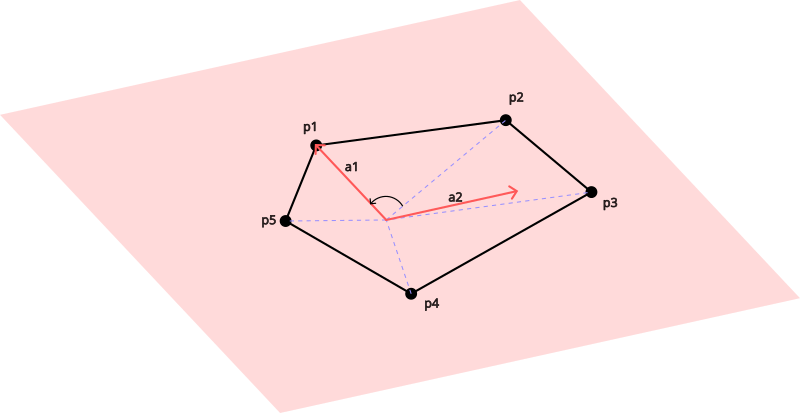
\includegraphics[width=0.5\linewidth]{plane}
    \caption{A figure showing an example Voronoi cell. Each point is labelled, and the position vectors are shown.}
    \label{fig:planeVoro}
\end{figure}

\begin{table}[h]
    \centering
    \begin{tabular}{llll}
    \hline
    Point & Angle & sign($a_2 \cdot P_i$) & Final angle \\ \hline
    p1             & 0              & +                 & 0                               \\
    p2             & 60             & +                 & 60                              \\
    p3             & 95             & +                 & 95                              \\
    p4             & 175            & -                 & 185                             \\
    p5             & 80             & -                 & 280                             \\ \hline
    \end{tabular}
    \caption{The first column refers to the point label and is a reference to figure \ref{fig:planeVoro}. The second column is the result of applying equation \ref{eq:angle}. The third column shows the sign of the projection of vector $P_i$ onto the second basis vector. The fourth column shows the angle after adjustment. The fourth column is calculated as: $360 - Angle$.}
    \label{tab:angles}
\end{table}

